\documentclass[a4paper,11pt]{article}
\usepackage[utf8]{inputenc}
\usepackage{algorithmic}
\usepackage{algorithm}
\usepackage{pst-plot}
\usepackage{graphicx}
\usepackage{endnotes}
\usepackage{graphics}
\usepackage{floatflt}
\usepackage{wrapfig}
\usepackage{amsfonts}
\usepackage{amsmath}
\usepackage{verbatim}
\usepackage{hyperref}
\usepackage{multirow}
\usepackage{pdflscape}
\usepackage{enumitem}
\usepackage[normalem]{ulem}

\usepackage{hyperref}
\hypersetup{pdfborder={0 0 0 0}}

\pdfpagewidth 210mm
\pdfpageheight 297mm 
\setlength\topmargin{0mm}
\setlength\headheight{0mm}
\setlength\headsep{0mm}
\setlength\textheight{250mm}	
\setlength\textwidth{159.2mm}
\setlength\oddsidemargin{0mm}
\setlength\evensidemargin{0mm}
\setlength\parindent{7mm}
\setlength\parskip{0mm}

\newenvironment{exercise}[3]{\paragraph{Exercise #1: #2 (#3pt)}\ \\}{
\medskip}
\newcommand{\question}[2]{\setlength\parindent{0mm}\ \\$\mathbf{Q_#1:}$ #2\ \\}

\author{\large{Ardi Tampuu, Tambet Matiisen, Raul Vicente}}
\title{\huge{Introduction to Computational Neuroscience}\\\LARGE{Practice session on Artificial Neural Networks}}

\begin{document}
\maketitle

\textbf{A request:} Please track how long it will take to complete this set of exercises. Add this time to your final report.
\ \\

\textbf{For Pyhton users:} You can do this task with any neural network package you want (sklearn, Keras, Neon, Caffe). But to save your time - it is really easy to run the code in Matlab/Octave.\\
\ \\
\ \\
\ \\
%
% Intro
%
In this session we are going to have a brief look on artificial neural networks. We start with simplest artificial neuron model called perceptron. Then we will see how simple feed-forward neural networks can be thought of as universal function approximators and what their limitations are. Finally we will use artificial neural network to predict rat's location like we did in Machine Learning practice session.

%
% Perceptron
%
\begin{exercise}{1}{Perceptron}{1}

\begin{wrapfigure}{r}{0.3\textwidth}
	\centering
	\vspace{-12pt}
	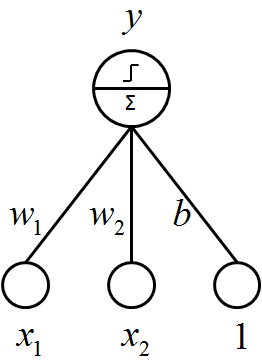
\includegraphics[width=0.22\textwidth]{perceptron.png}
	\caption{Simple perceptron}
	\label{fig:perceptronexample}
	\vspace{-5pt}
\end{wrapfigure}

Perceptron is the simplest artificial network model invented by Frank Rosenblatt in late 1950s. He added a learning rule to McCulloch-Pitts neuron, that allows it to learn certain functions from example inputs and outputs.

Perceptron works on binary data – both its inputs $x_j$ and output $y$ are ones or zeros. Output 1 or 0 can be thought of as binary classification – whether object represented by the given input belongs to certain class or not. 

Perceptron’s weights $w_j$ can be any real numbers. Its prediction is calculated with following formula:

$$
y = \left\{
	\begin{array}{l l}
		1, \text{if } x_1 w_1 + ... + x_m w_m + b \geq 0\\
		0, \text{otherwise}
	\end{array}
	\right.
$$

Here $b$ is the bias term, that is added to the sum. In practice it is easier to just add additional input, which is always one. Then we don’t have to treat bias as something special, it is just an additional weight to learn. Learning rule for the perceptron is very simple:

$$
w_j = w_j + (t_i - y_i) x_{ij}
$$

Index $i$ is used to denote $i$-th example data point. Learning rule must be applied for all data points and for each weight. You will continue updating the weights until all data points are classified correctly.

It turns out, that perceptron is always able to successfully learn a classification rule for datasets, which are \textit{linearly separable} -- data points with label 1 and label 0 can be separated by a line (in case of two inputs), plane (in case of three inputs) or hyperplane (in case of input of any dimensionality). If the dataset is not linearly separable, perceptron will never \textit{converge} (settle to a certain set of weight values). \newline

Example code for this exercise is in \texttt{perceptron.m}. Your task is to fill in the perceptron learning rule and decide for four example datasets (replace the dataset number on line 12) if they are linearly separable or not. Of course, in 2D one can do this by just looking at the data, but in higher dimensional data this would not be the case. In your report you must include the final image with the decision boundary (the black line) for all four datasets. \footnote{\textbf{Decision boundary} is a line (plane/hyperplane) that separates the positive and negative datapoints - positives will be one one side and negatives on the other side} For linearly separable datasets also add the approximate number of steps it took for the perceptron to convergence (to reach 0 errors).

\end{exercise}

%
% Sinusoid
%
\begin{exercise}{2}{Function Approximation}{1.5}

Universal Approximation Theorem states that any continuous function can be approximated to any desired precision by a feed-forward network with a single hidden layer containing a finite number of non-linear neurons. In practice this theorem is of no use, because:
\begin{itemize}
  \item it states only, that these functions can be \uline{represented} by feed-forward network with one hidden layer. The theorem doesn’t say anything about if this approximation is \uline{learnable} - if with our current algorithms we can find the necessary weight values;
  \item the construction used in the proof uses a huge number of neurons in the hidden layer. This would be unreasonable for any practical application;
  \item as the theorem doesn’t consider learnability, it also doesn’t state anything about how well the networks generalizes to samples beyond its training data.
\end{itemize}

Nevertheless the theorem is a nice concept to guide your thinking – if some problem can be described as a function calculating output based on several inputs, then it probably can be approximated reasonably well with an artificial neural network.\newline

\begin{wrapfigure}{r}{0.3\textwidth}
	\centering
	\vspace{-12pt}
	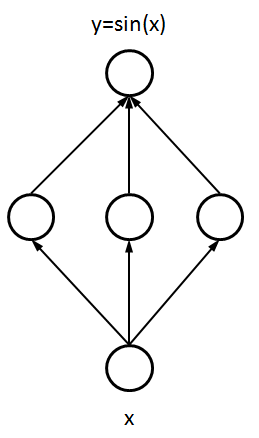
\includegraphics[width=0.20\textwidth]{sine.png}
	\label{fig:sineexample}
	\vspace{-5pt}
\end{wrapfigure}

In this task we are going to approximate sine function using a neural network. This neural network is very simple – it consists of just one input node (the $x$ value), several hidden nodes and one output node ($y = sin(x)$).

Hidden nodes use sigmoid activation function to achieve non-linearity (the nodes apply sigmoid function to the weighted sum of their inputs). Output node is linear, no activation function is applied. Loss function is simply squared error:

$$
L = \frac{1}{2n}\sum_{i=1}^{n} (target_i - predicted_i)^2
$$

It calculates average loss over all $n$ data points in the training set. \newline

For creating neural networks we are making use of DeepLearnToolbox toolkit by Rasmus Berg Palm. The tookit is already included with your download in folder \texttt{DeepLearnToolbox}. Feel free to explore the source in \texttt{DeepLearnToolbox/NN} folder, it is quite clean Matlab code.\newline


For this exercise you need to run the code in \texttt{sinusoid.m} with different number of nodes and answer the questions.

\question{1}{First run the \texttt{sinusoid.m} exactly as it is. The script creates a neural network that tries to approximate the sine function between $-2\pi\ and\ 2\pi$, based on 20 training data points. The neural network has 5 hidden nodes. All the weights and biases are initialized with random values. It would be best if you understand more of less what the code does (read the comments).
Notice that the script will generate a plot that shows the true shape of the sine, the training data points, and the current approximation made by the network. This plot is updated as we pass over the training data and learn the weights. After the learning has finished another plot appears, summarizing how the loss decreased during training. Add the two plots to the report. Answer the following questions:
\begin{itemize}
\item Does the neural network represent the function well within the range $-2\pi\ to\ 2\pi$? If not, how many of the curves of the sine does the network manage to capture well? (In some cases (especially in Matlab) it might capture the shape well, but if you run it many times it mostly shouldn't) 
\end{itemize}
}
\question{2}{Now run the script \texttt{minimal\_sinusoid.m}. In this script we also have a network of 5 nodes, but the weights and biases are not initialized randomly, but with useful values given by me (not learned by an algorithm). In this case you should see that the network learns to capture the shape of the sine really well. As you can see - the function can be represented well by a 5-node network, but the learning algorithm we used in Q1 did not allow us to find this approximation. 
\begin{itemize}
\item Hypothesize why doesn't the network always learn a good solution if we start with randomly initialized weights. In here uncommenting the line  \texttt{plot\_sinusoid\_components(test\_x,nn)} for the  two cases might provide insights.
\item How good is the network at extrapolation (predicting values outside the range it had training data for)? Why is that not surprising? 
\end{itemize}
}
\question{3}{Increase the number of hidden nodes in \texttt{sinusoid.m}, by replacing the number 5 with the desired number on line 28. 
\begin{itemize}
\item How many hidden nodes do you need so that starting from randomly initalized parameters the learning algorithm would converge to a good representation of the function (training loss$<0.1$). Run the code couple of times for each tested number of nodes and report the result if at least one trial is good. Add the plot with the datapoints and the approximation.
\end{itemize}
}
\end{exercise}

%
% MNIST
%
\begin{exercise}{3}{Rat position decoding}{1.5pt + 1.0pt + some bonus }

Finally we will use artificial neural network to predict a rat's location based on the recordings from its hippocampal neurons. Remember that in the Machine Learning practice session we worked with this dataset and linear discriminant analysis gave us an accuracy of around 35\% on test set. 

For neural networks we are once again making use of DeepLearnToolbox toolkit.

This time our network has 71 inputs that are the spike counts in different neurons during a period of time. In this first part of the task we divide the space into 16 squares and predict in which region the rat is located (like we did in ML practice). This means the network has 16 outputs, each of which is a probability corresponding to one of the squares. Between the inputs and outputs we have one or more layers of hidden nodes with hyperbolic tangent nonlinearity. In order to guarantee that the 16 output probabilities sum up to 1, we use a function called softmax (Google it if interested). When teaching the network to predict the correct zone we minimize the cross-entropy loss (see lecture).

After you have run the code and got initial results, your goal is to improve classification accuracy. For that you would need to tune learning rate, number of hidden nodes, number of epochs (iterations over full data set) and other parameters. Finding good parameters for neural networks can be quite tedious and frustrating, so I will not ask you to do it, instead we will do it together:

\begin{enumerate}
  \item We start by modifying the \textbf{learning rate}. This parameter decides how big a step will we take in the direction of the gradient during gradient descent. With learning rate too high, our model will never converge. With LR too low, the model will take too long time to reacha  good solution and is also prone to getting stuck in a bad local minima. Try $LR=1$ first and see that the loss graph is not stable - there are major zig-zags. This indicates that the learning rate is too high. Next we try 0.1. Still jumpy, but a little bit better. Finally we try 0.01 - very smooth, but error goes down a lot slower. Add all plots and the prediction accuracies after 30 epochs (the code prints it out) to the report. Which LR would you choose (there is no absolute truth, so explain your choice)? Compare the results with baseline (LDA accuracy).
  \item \textbf{Momentum} is a method that that allows better and more stable learning by remembering the global trends in weight changes - if all previous datapoints have suggested that a weight should be lowered, we decrease it faster than normal. If datapoints do not agree on how to change a certain weight, we change it only slowly. \newline Set the value of momentum to 0.95. Run the code with LR=0.1 and LR=0.01 (you can even try 0.001). Which LR you judge more adequate now (there is no absolute truth, so explain your choice)?
  \item With momentum 0.95 and LR 0.01 you should see \textbf{overfitting}, which means that network learns to predict well on training examples, but this knowledge doesn't generalize to the test set. You can detect this from large gap between training and validation misclassification rate. To fight against overfitting we have two tools - the weight penalty and dropout. 
If we brought in weight penalty, we would again need to search for a good learning rate. So instead we use dropout (in this case you might need to increase the number of nodes, but that's the next bulletpoint). Dropout means that at every training step we do not consider some nodes (a certain proportion) in our network - we simply do as if they were not there. In every training step the left out neurons are different. Dropout is so effective because it is similar to adding random noise to the network - it makes it impossible to simply remember the training data and forces the model to generalize. It also has similarity with ensembling techniques.\newline Your task is to try \textbf{dropout} percentages 0.2, 0.4, 0.6 and see if you can bring the validation error down (making the difference with training error smaller is not enough - only thing we care about is the validation accuracy). Add plots to the report.
    \item Once you have stabilized the learning, try to increase \textbf{number of hidden nodes} and see if testing error improves. You can also add more layers by simply adding a number in nnsetup - for example \texttt{$nn\ =\ nnsetup([71\ 100\ 100\ 16]);$}  creates two layers of 100 nodes. More layers might sound appealing, but it makes the learning slower to converge, so be cautious with it. Add the plots and accuracies that you achieved with bigger networks.
  \item Finally, if the loss for test set seems to still decrease at the end of training (end of 30 epochs), increase the \textbf{number of epochs} and see how low the error can go. Usually it plateaus at some point and there is no reason to train further. (no task in particular in here)
  \item \textbf{Your final task is} to get the validation accuracy above 0.42. There will be bonus points for the ones that get the best accuracy (it's a competition!).
\end{enumerate}

-----------------------------------------------------

In the second part of this exercise we will not predict the 16 areas where the rat is in, but the XY coordinates directly. This means we have 2 linear output nodes (nodes with no nonlinearity) predicting the coordinates rather than 16 outputs predicting probabilities (using softmax). When training the network we minimize the squared difference between true coordinates and the predicted coordinates (mean squared error loss).

\begin{itemize}
\item Run the code \texttt{rat\_regression.m}. The program outputs the baseline error (how wrong the prediction is on average when using a linear model). After training a network the script will also print out how big is the average error made by the neural network. Report the two values and which model is better. Add the plot of how error changed during training. Notice that the error on the graph (the thing we minimize) is mean squared error (MSE), whereas we finally care about mean distance.
\item Try to improve the result (get lower error). Make a hypothesis of what could help you - more neurons? higher or lower dropout? different learning rate? Write down your hypothesis, run the models and report if it worked out or not. It is absolutely not important that you actually improve the result. The task is to explore. HINT: change only one parameter at a time, otherwise you will not know which change caused the benefit/problem. You need to report at least 3 different things you tried.
\item Again bonus points for the people who achieve the lowest error.
\end{itemize}
\end{exercise}




\ \\
\ \\
\ \\
\ \\
\ \\
Please submit a \texttt{pdf} report with answers to the questions and comments about your solutions. YOU MUST INCLUDE THE CODE. Please mark how long it took to complete this set of exercises. Upload a zip/rar/etc with the \texttt{pdf} and the code to the practice session page on the course website.

\end{document}
